\input preamble_DPO.tex

\date{20 января 2021}		% Дата семинара
\setcounter{s}{2}			% Номер семинара

\begin{document}


\title{Дискретная математика:\\
комбинаторика и вероятность}

\institute{Факультет компьютерных наук, НИУ ВШЭ}

\begin{frame}
  \titlepage
\end{frame}


\begin{frame}{Мощность множества}

\defn \acc{Мощностью} конечного множества $A$ называется количество элементов в нем. Обозначение: $|A|$.

\exmpl Среди математиков каждый седьмой -- философ, а среди философов каждый девятый -- математик. Кого больше: философов или математиков?


\acc{Правило суммы:} если конечные множества $A$ и $B$ не пересекаются,
то мощность их объединения равна сумме мощностей
$$|A \cup B|=|A|+|B|,\quad \text { если } A \cap B=\varnothing.$$
Если же пересечение $A$ и $B$ не пусто, то
$$|A \cup B|=|A|+|B|- |A \cap B|.$$
\exmpl Найдем количество не превосходящих $100$ натуральных чисел, делящихся на два или три.


\end{frame}


\begin{frame}{Мотивировка определения вероятности}


\exmpl При броске кубика может выпасть одна из шести граней. Какова вероятность выпадения $\geqslant 5$ очков?

\exmpl Подбросим монету дважды.
Какова вероятность выпадения двух орлов?


\end{frame}


\begin{frame}{Определение классической вероятности}

\defn \acc{Пространство элементарных исходов} — множество $\Omega$ всех исходов случайного эксперимента.

Если все исходы имеют одинаковую вероятность, то такое $\Omega$ называется пространством с \acc{равновероятными элементарными исходами}.

\defn Всякое подмножество $\Omega$ называется \acc{cобытием}.

\defn Если $\Omega$ --- пространством с равновероятными элементарными исходами, то \acc{вероятностью события} $A$ называется отношение $P(A)=\dfrac{|A|}{|\Omega|}.$

\exmpl При броске кубика $\Omega=\{1,2,3,4,5,6\}.$

Событие $A$ -- <<на кубике выпало $\geqslant 5$ очков>>, $A=\{5,6\},$ $P(A)=\dfrac{2}{6}=\dfrac 13.$

\end{frame}

\begin{frame}{Два броска кубика}

\exmpl При двукратном броске монетки $\Omega=\{OO,OP,PO,PP\}.$ 

Событие $B$ -- <<выпало два орла>>, $B=\{OO\},$ $P(B)=\dfrac{1}{4}$.

\exmpl Игральный кубик бросают дважды. Какова вероятность, что сумма очков за два броска будет равняться $7$?

\end{frame}

\begin{frame}{Два броска кубика}

$$\Omega= \left\lbrace\begin{array}{c c c c c c }
(1,1), & (1,2), & (1,3), & (1,4), & (1,5), & (1,6), \\
(2,1), & (2,2), & (2,3), & (2,4), & (2,5), & (2,6), \\
(3,1), & (3,2), & (3,3), & (3,4), & (3,5), & (3,6), \\
(4,1), & (4,2), & (4,3), & (4,4), & (4,5), & (4,6), \\
(5,1), & (5,2), & (5,3), & (5,4), & (5,5), & (5,6), \\
(6,1), & (6,2), & (6,3), & (6,4), & (6,5), & (6,6) \\
\end{array}\right\rbrace$$

Тогда таблица сумм выглядит так:

\begin{center}
\renewcommand{\arraystretch}{1.1}
\setlength{\tabcolsep}{15pt}
\begin{tabular}{|c|c|c|c|c|c|}
\hline 2 & 3 & 4 & 5 & 6 & 7 \\
\hline 3 & 4 & 5 & 6 & 7 & 8 \\
\hline 4 & 5 & 6 & 7 & 8 & 9 \\
\hline 5 & 6 & 7 & 8 & 9 & 10 \\
\hline 6 & 7 & 8 & 9 & 10 & 11 \\
\hline 7 & 8 & 9 & 10 & 11 & 12 \\
\hline
\end{tabular}
\end{center}

\end{frame}

\begin{frame}{Два броска кубика}

Пусть $A$ ---  событие <<сумма очков за два броска равняется $7$>>. 

Тогда $P(A)=\dfrac{|A|}{|\Omega|}=\dfrac{6}{36}=\boxed{\dfrac 16}.$


\exmpl Чему равняется $|\Omega|$ для $4$ или $10$ бросков кубика?


\end{frame}

\begin{frame}{Правило произведения}


\acc{Правило произведения:} если объект первого типа можно выбрать $n_1$ способами, после чего второй объект можно выбрать $n_2$ способами и т.д.
($k$-ый объект можно выбрать $n_k$ способами), то выбрать последовательно $k$ объектов можно $n_1 \times n_2 \times \ldots \times n_k$ способами.

\exmpl Найдём количество трехзначных чисел с помощью правила
произведения.

\exmpl Сколькими способами можно выбрать командира и его заместителя в отделении из $10$ человек?

\defn Количество способов выбрать упорядоченный набор $k$ элементов из $n$-элементного множества называется \acc{числом размещений} из $n$ по $k$ и обозначается

$$A_n^k=n(n-1)\dots(n-(k-1))=\frac{n!}{(n-k)!}$$


\end{frame}


\begin{frame}{Задача де Мере}

\exmpl Игральный кубик бросают четыре раза. Какова вероятность выпадения  хотя бы одной шестерки?

$$|\Omega|=6^4.$$

Пусть $A_6$ -- событие <<хотя бы раз выпала шестерка>> =$a$.

Рассмотрим $\neg a$=<<шестерка ни разу не выпала>>. Ему соответствует множество $\Omega\setminus A_6$.

Но <<шестерка ни разу не выпала>> = <<выпадали только 1,2,3,4 или 5>> $\Longrightarrow$ по правилу произведения, $|\Omega\setminus A_6|=5^4$.

Тогда $|A_6|=|\Omega|-|\Omega\setminus A_6|=6^4-5^4$ (правило суммы).

$$P(A_6)=\dfrac{|A_6|}{|\Omega|}=\dfrac{6^4-5^4}{6^4}=1-\left(\dfrac{5}{6}\right)^4\approx \boxed{0,5177\ldots}$$

\end{frame}


\begin{frame}{Вероятность отрицания}

\acc{Вероятность отрицания к событию:} если $A$ -- некоторое событие, а $\bar{A}=\Omega\setminus A$ -- отрицание к нему, то 

$$\acc{\boxed{P(A)=1-P(\bar{A})}}$$


\end{frame}



\begin{frame}{Неравновероятные элементарные исходы}

Не все ситуации можно описать равновероятной моделью.

Пусть $\Omega=\{ \omega_1,\omega_2, \omega_3,\ldots \}$ --- пространство элементарных исходов.

Сопоставим каждому элементарному событию $\omega_i$ его вероятность $P(\omega_i)=p_i$, $0\leqslant p_i\leqslant 1$ так, чтобы 
$$p_1+p_2+p_3+\ldots=1.$$
\defn $P$ называется \acc{функцией вероятности}.

\defn \acc{Конечное вероятностное пространство} --- это пространство элементарных событий $\Omega$ вместе с функцией вероятности $P$ на нём.

\defn \acc{Вероятность события} --- сумма вероятностей всех его элементарных исходов.

\end{frame}

\begin{frame}{Дерево событий}

\exmpl Для прохождения в следующий тур команде необходимо выиграть два раза подряд в серии из трёх игр.

Вероятность выиграть в первом матче равна $\frac 12$. Вероятность выигрыша после победы в предыдущем матче возрастает до $\frac 23$, а после поражения уменьшается до $\frac 13$.

Каковы шансы у команды пройти в следующий тур?

Когда задача состоит из цепочки событий, но элементарных исходов не так много, для решения удобно использовать \acc{дерево событий}.

\end{frame}

\begin{frame}{Дерево событий}

\begin{center}
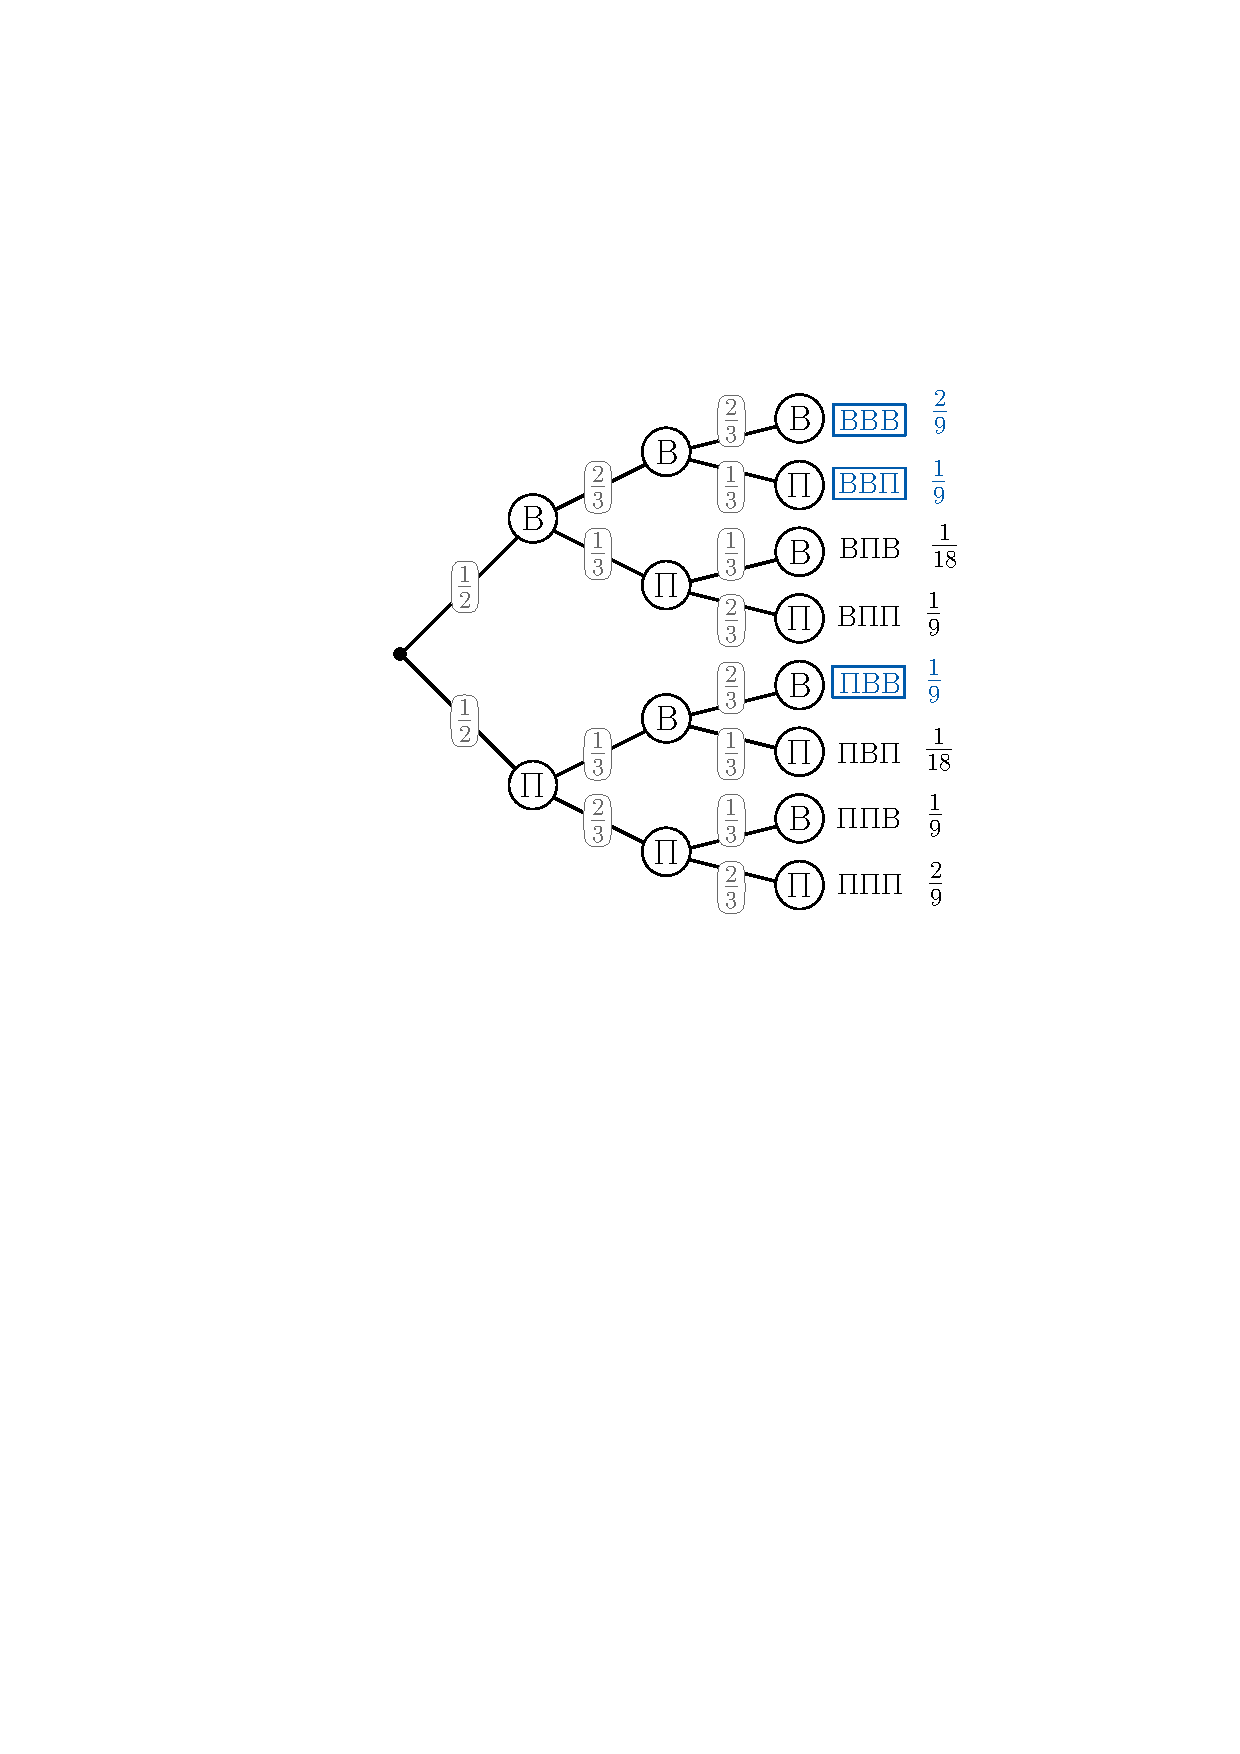
\includegraphics[width=\textheight]{img/tree000.pdf}
\end{center}

\end{frame}

\begin{frame}{Дерево событий}

Дерево событий задает $\Omega$.
$$\Omega=\{\text{ВВВ},\text{ВВП},\text{ВПВ}, \ldots\}.$$

Сумма всех вероятностей в последнем столбце равняется единице.

Пусть событие $A$ --- "команда прошла в следующий тур".

Наша задача --- найти $P(A)$.

$$P(A)=\frac{2}{9}+\frac{1}{9}+\frac{1}{9}=\boxed{\frac{4}{9}}$$

\end{frame}


\begin{frame}{Число сочетаний}

\exmpl Скольким способами можно из десяти сотрудников выбрать двух для выдачи им премии? А трех?

\defn Количество способов выбрать $k$-элементное подмножество из $n$ элементного множества называется \acc{числом сочетаний} из $n$ по $k$
$$\acc{\boxed{ \binom {n}{k}=C_n^k=\dfrac{n!}{k!(n-k)!}}}$$

\end{frame}




\begin{frame}{Симметричная схема Бернулли}

\exmpl Вероятность выпадения ровно трех решек при подбрасывании симметричной монеты четыре раза равняется

$$P(X=3)=\binom {4}{3} \cdot \left(\frac 12\right)^4=\boxed{\frac 14}.$$

\exmpl Вероятность выпадения ровно $50$ решек при подбрасывании симметричной монеты $100$ раз равняется
$$P(X=50)=\binom {100}{50}\cdot \left(\frac 12\right)^{100} \approx \boxed{0.0796\ldots}$$

\end{frame}

\begin{frame}{Наивероятнейшее число успехов}

Проверим интуицию: чему равняется вероятность выпадения не более $25$ решек при подбрасывании монеты $100$ раз?

Варианты ответа:
$P(X\leqslant 25)$
\begin{itemize}
\item больше $\frac 12$;
\item меньше $\frac 12$, но больше $\frac{1}{10}$;
\item меньше $\frac{1}{10}$, но больше $\frac{1}{100}$;
\item меньше $\frac{1}{100}$, но больше $\frac{1}{1000}$;
\item меньше $\frac{1}{1000}$, но больше $\frac{1}{1000000}$;
\item меньше $\frac{1}{1000000}$.
\end{itemize}

\end{frame}

\begin{frame}{Наивероятнейшее число успехов}

Давайте посчитаем:
$$P(X\leqslant 25)=$$
$$=P(X=0)+P(X=1)+\ldots+P(X=25)=$$
$$=\binom {100}{0}\left(\frac{1}{2}\right)^{100}+\binom {100}{1}\left(\frac{1}{2}\right)^{100}+\ldots+\binom {100}{25}\left(\frac{1}{2}\right)^{100}\approx$$
$$\approx \boxed{2.818\ldots \times 10^{-7}}< \frac{1}{1000000}!$$

\end{frame}



\begin{frame}{Схема Бернулли}{Дополнительный материал}

\defn \acc{Схемой Бернулли} называется последовательность из $N$ независимых испытаний с двумя возможными исходами, которые обычно обозначают $1$ и $0$ (<<успех>> и <<неудача>>, или
<<орел>> и <<решка>>). Причем $P(1)=p,\ P(0)=1-p$.

Пространство элементарных событий $\Omega$ состоит из всех возможных последовательностей $1$ и $0$ длины $N$. 

\begin{align*}
\Omega=\{\omega=(\omega_1,\ldots,\omega_N)\ |\ \omega_i =0 \text{ или } 1, i=1,\dots,N \}.
\end{align*}

Вероятность исхода $\omega$, в котором произошло $k$ <<успехов>> и $N-k$ <<неудач>> равняется $P(\omega)=p^k(1-p)^{N-k}.$


\end{frame}

\begin{frame}{Случайная величина}{Дополнительный материал}

\defn \acc{(Дискретная) случайная величина } --- функция из множества $\Omega$ в $\RR$.

\exmpl Случайная величина $X$ --- количество успехов из $N$ испытаний в схеме Бернулли.

Чему равняется $P(X=k)$?

\end{frame}

\begin{frame}{Схема Бернулли}{Дополнительный материал}

Значению $X=k$ соответствует событие $A_k$, состоящее из всех с исходов $k$ успехами.

Вероятность каждого исхода $A_k$ равняется $p^k(1-p)^{N-k}$.

Всего исходов ровно с $k$ успехами $C_N^k$ (количество способов выбрать места для $k$ единичек).

Тогда $$P(X=k)=P(A_k)=\acc{\boxed{C_N^k \cdot p^k(1-p)^{N-k}}}$$

\end{frame}


\begin{frame}{Семинарская часть}

\z Есть 3 гвоздики, 4 розы и 5 тюльпанов.

\p Сколькими способами можно составить букет из цветов одного вида?

\p Сколькими способами из них можно составить букет, в котором нечетное количество цветов каждого вида?

\p Сколькими способами можно составить букет, используя любые из
имеющихся цветов?

(Цветы одного сорта считаем одинаковыми, количество цветов в букете не ограничено, но не равно 0.)

\z На плоскости отмечено $10$ точек так, что никакие три из них не лежат на одной прямой. Сколько существует треугольников с вершинами в этих точках?

%\z Сколько существует 9-значных чисел, цифры которых расположены в порядке убывания (то есть каждая следующая меньше предыдущей)?

\end{frame}

\begin{frame}{Семинарская часть}

\z Найдите вероятность события <<при броске двух кубиков выпало не
менее $8$ очков>>.

\z Найдите вероятность события <<при бросании 6 монет выпало хотя бы $3$ орла>>.

\z Найдите вероятность того, что в случайном 4-буквенном слове в русском алфавите, есть хотя бы одна гласная? (Всего 33 буквы, 10 из них
гласные.)

\end{frame}

\begin{frame}{Семинарская часть}

\z В коробке лежит $6$ белых и $6$ черных шаров. Из нее по очереди достают три шара.

{\bf a)} Какова вероятность вынуть ровно $1$ черный шар?

{\bf б)} А хотя бы по одному черному и белому?


\z Готовясь к экзамену, студент должен подготовить ответы на две серии вопросов по $10$ вопросов в каждой. Он знает ответы на $9$ вопросов первой серии и на $8$ из второй. Надо ответить на три вопроса, два из которых выбираются экзаменатором из первой серии, а третий из второй. Найти вероятность, что студент ответит на все три вопроса.

\end{frame}

\begin{frame}{Семинарская часть}{Дополнительный материал}

\zh Работу портала онлайн магазина поддерживают $10$ серверов. В день акции нагрузка на сервера будет пиковой, и прогнозируется, что каждый сервер может выйти из строя с вероятностью $\nicefrac{1}{5}$. При этом нагрузка на оставшиеся сервера остается пиковой, и вероятность их выхода из строя не повышается. Какова вероятность, что после акции хотя бы два сервера останутся в строю?

\end{frame}

\begin{frame}{Парадокс Монти Холла}{Дополнительный материал}

Перед Вами три двери: за одной автомобиль, за двумя другими --- козы.

\vspace{-2mm}
\begin{center}
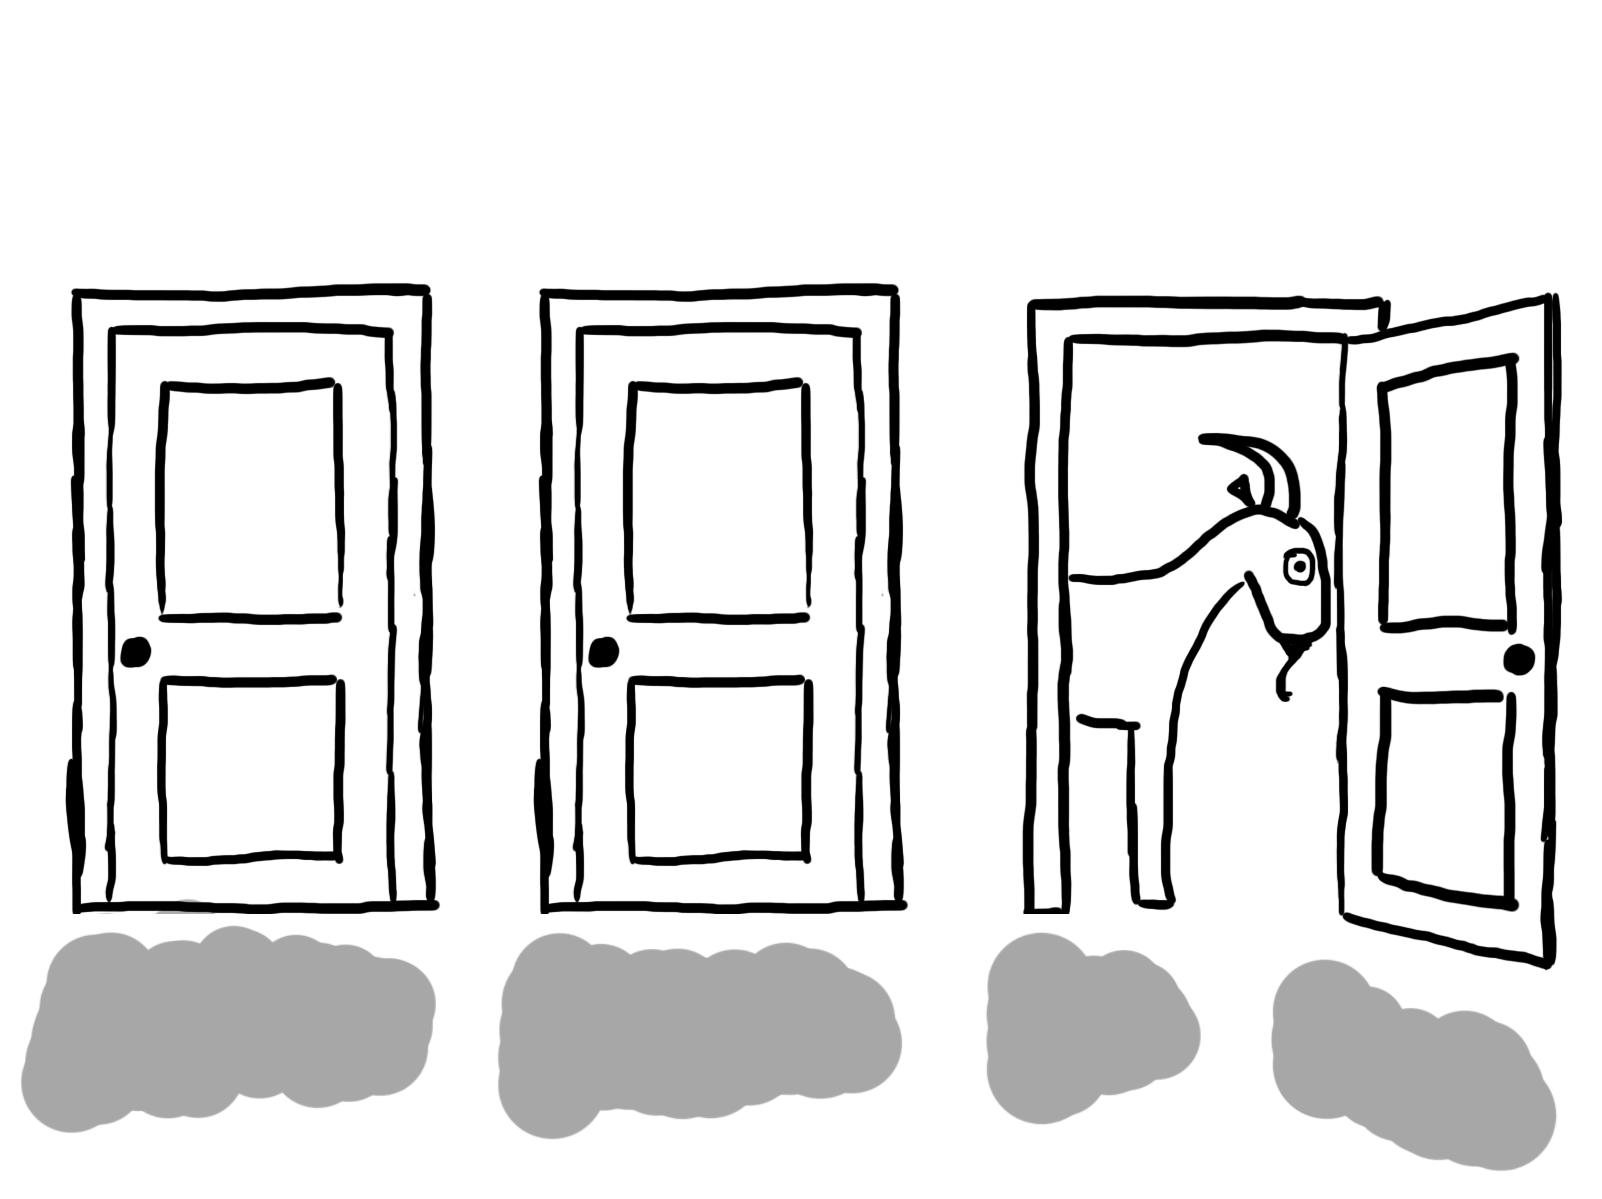
\includegraphics[width=40mm]{img/doors1-2.png}
\end{center}

Вы выбираете одну из дверей, но ведущий не говорит Вам, что за ней находится, а открывает другую дверь, за которой находится коза.

После этого он задает Вам вопрос: <<Измените ли Вы свой выбор?>>


\end{frame}


\begin{frame}{Парадокс Монти Холла}{Дополнительный материал}


Рассмотрим этот вопрос с точки зрения вероятности:

\z С какой вероятностью Вы выиграете автомобиль, если

{\bf 1)} не будете менять выбор;

{\bf 2)} измените выбор случайным образом;

{\bf 3)} измените свой выбор?



Мы будем решать задачу в предположении, что:

\begin{itemize}
\item автомобиль размещён за любой из дверей с одинаковой вероятностью;
\item ведущий знает, где находится автомобиль;
\item ведущий в любом случае открывает дверь с козой (но не ту, которую выбрал игрок) и предлагает игроку изменить выбор;
\item если у ведущего есть выбор, то он выбирает любую из двух дверей с одинаковой вероятностью.

\end{itemize}


\end{frame}


\begin{frame}{Парадокс Монти Холла}{Дополнительный материал}

\begin{itemize}

\item Если не менять выбор, то выиграть можно только в том случае, если с самого начала была выбрана дверь с автомобилем.

Победа обеспечена в $\nicefrac{1}{3}$ случаев.

\item Если изменить выбор случайным образом, то придется выбирать из двух дверей.

Победа обеспечена в половине случаев.

\item Если всегда менять свой выбор, то проиграть можно только в том случае, если в начале была выбрана дверь с автомобилем.

Победа обеспечена в $\nicefrac{2}{3}$ случаев.

\end{itemize}

Невероятно, но всегда стоит менять свой выбор!


\end{frame}


\end{document}


